\documentclass[12pt,a4paper]{article}
\usepackage[a4paper, margin=0.8in, headheight=14pt]{geometry}
\usepackage{fontspec}
\usepackage{unicode-math}
\setmainfont{TeX Gyre Pagella}
\setmonofont[Scale=0.88]{TeX Gyre Cursor}
\setmathfont{Latin Modern Math}
\usepackage{xcolor}
\usepackage{colortbl}
\usepackage{titlesec}
\usepackage{enumitem}
\usepackage{tabularx}
\usepackage{booktabs}
\usepackage{array}
\usepackage{amsmath}
\usepackage{tikz}
\usetikzlibrary{shapes.geometric, arrows.meta, positioning, calc, fit, decorations.pathreplacing, decorations.pathmorphing, patterns, backgrounds}
\usepackage[american]{circuitikz}
\usepackage{tcolorbox}
\tcbuselibrary{skins, breakable}
\usepackage{etoolbox}
\usepackage{hyperref}
\usepackage{fancyhdr}
\usepackage{graphicx}
\usepackage{microtype}
\hyphenpenalty=10000
\exhyphenpenalty=10000
\sloppy
\usepackage{caption}
\usepackage{setspace}
\usepackage{multirow}
\usepackage{tocloft}
\newcommand{\Q}[1]{\textbf{#1}\par\noindent\ignorespaces}
\definecolor{myred}{RGB}{196,30,58}
\definecolor{mydark}{RGB}{30,30,50}
\definecolor{mygreen}{RGB}{14,120,80}
\definecolor{myteal}{RGB}{0,130,140}
\definecolor{myamber}{RGB}{180,100,0}
\definecolor{mypurple}{RGB}{100,30,160}
\definecolor{mygray}{RGB}{246,247,249}
\definecolor{mgframe}{RGB}{180,185,200}
\definecolor{watermark}{RGB}{145,150,170}
\definecolor{hdrred}{RGB}{250,232,235}
\definecolor{hdrgreen}{RGB}{220,244,233}
\definecolor{hdrteal}{RGB}{220,242,244}
\definecolor{hdramber}{RGB}{253,242,215}
\definecolor{hdrpurple}{RGB}{238,228,255}
\definecolor{hdrgray}{RGB}{238,240,245}
\definecolor{rowalt}{RGB}{250,251,253}
\AfterEndEnvironment{tcolorbox}{\color{mydark}}

\titleformat{\section}{\large\bfseries\color{myred}}{\thesection.}{0.5em}{}[\vspace{1pt}{\color{myred}\rule{\linewidth}{0.8pt}}]
\titleformat{\subsection}{\normalsize\bfseries\color{myteal}}{\thesubsection}{0.5em}{}
\titlespacing*{\section}{0pt}{18pt}{7pt}
\titlespacing*{\subsection}{0pt}{11pt}{4pt}
\setlength{\parindent}{0pt}
\setlength{\parskip}{4pt}
\renewcommand{\cfttoctitlefont}{\large\bfseries\color{myred}}
\renewcommand{\cftaftertoctitle}{\par\noindent{\color{myred}\rule{\linewidth}{0.8pt}}}
\setlength{\cftbeforetoctitleskip}{0pt}
\setlength{\cftaftertoctitleskip}{6pt}
\renewcommand{\cftsecfont}{\normalsize\bfseries\color{mydark}}
\renewcommand{\cftsecpagefont}{\normalsize\bfseries\color{mydark}}
\renewcommand{\cftsecleader}{\cftdotfill{\cftdotsep}}
\setlength{\cftbeforesecskip}{7pt}
\renewcommand{\cftsubsecfont}{\small\color{mydark}}
\renewcommand{\cftsubsecpagefont}{\small\color{mydark}}
\setlength{\cftbeforesubsecskip}{3pt}
\setlength{\cftsubsecindent}{1.4em}
\renewcommand{\cftpartfont}{\normalsize\bfseries\color{myteal}}
\renewcommand{\cftpartpagefont}{\normalsize\bfseries\color{myteal}}
\setlength{\cftbeforepartskip}{14pt}
\renewcommand{\arraystretch}{1.45}
\setlength{\tabcolsep}{6pt}
\arrayrulecolor{mydark}
\newcolumntype{B}[1]{>{\small\bfseries\raggedright\arraybackslash}m{#1}}
\newcolumntype{C}[1]{>{\centering\arraybackslash}m{#1}}
\newcolumntype{Y}{>{\small\raggedright\arraybackslash}X}
\renewcommand{\tabularxcolumn}[1]{m{#1}}
\newcommand{\currmodule}{Module 1}
\pagestyle{fancy}
\fancyhf{}
\fancyhead[L]{\small\color{myred}\textbf{OE-EC804A}\;\color{mydark}--- Artificial Intelligence}
\fancyhead[R]{\small\color{myteal}\textbf{\currmodule\ Notes}}
\fancyfoot[C]{\small\color{mydark}\thepage}
\fancyfoot[R]{\small\color{watermark}\textit{\copyright\ Biraj}}
\renewcommand{\headrulewidth}{0.5pt}
\renewcommand{\footrulewidth}{0.3pt}

\hypersetup{colorlinks=true, linkcolor=myteal, urlcolor=myteal,
  pdfauthor={Biraj Sarkar},
  pdftitle={OE-EC804A --- Combined Notes}}

\tcbset{
  tikzbox/.style={colback=mygray, colframe=mgframe, boxrule=0.6pt, arc=4pt,
    left=8pt, right=8pt, top=6pt, bottom=6pt,
    colbacktitle=mgframe, coltitle=mydark, fonttitle=\small\bfseries, unbreakable},
  defbox/.style={colback=hdrgreen, colframe=mygreen, boxrule=0.8pt, arc=4pt,
    left=9pt, right=9pt, top=6pt, bottom=6pt,
    colbacktitle=mygreen, coltitle=white, fonttitle=\small\bfseries},
  formulabox/.style={colback=hdrteal, colframe=myteal, boxrule=0.8pt, arc=4pt,
    left=9pt, right=9pt, top=7pt, bottom=7pt,
    colbacktitle=myteal, coltitle=white, fonttitle=\small\bfseries},
  examplebox/.style={colback=hdramber, colframe=myamber, boxrule=0.8pt, arc=4pt,
    left=9pt, right=9pt, top=6pt, bottom=6pt,
    colbacktitle=myamber, coltitle=white, fonttitle=\small\bfseries},
  masonbox/.style={colback=hdrpurple, colframe=mypurple, boxrule=0.8pt, arc=4pt,
    left=9pt, right=9pt, top=6pt, bottom=6pt,
    colbacktitle=mypurple, coltitle=white, fonttitle=\small\bfseries},
  exambox/.style={colback=hdrpurple, colframe=mypurple, boxrule=1pt, arc=5pt,
    left=10pt, right=10pt, top=8pt, bottom=8pt,
    colbacktitle=mypurple, coltitle=white, fonttitle=\bfseries,
    breakable, title after break={\textbf{Frequently Asked / Viva Questions (contd.)}}}
}
\tcbset{breakable}
\tcbset{coltext=mydark}
\tcbset{after={\color{mydark}}}

\tikzset{
  block/.style={rectangle, draw=myteal, fill=hdrteal,
    text width=2.4cm, align=center, minimum height=0.95cm,
    font=\small, rounded corners=3pt, line width=0.7pt},
  redblock/.style={rectangle, draw=myred, fill=hdrred,
    text width=2.4cm, align=center, minimum height=0.95cm,
    font=\small, rounded corners=3pt, line width=0.7pt},
  arrow/.style={-Stealth, thick, color=mydark},
  line/.style={thick, color=mydark},
  sblock/.style={circle, draw=myteal, fill=hdrteal, minimum size=0.8cm, font=\small\bfseries},
  goalblock/.style={circle, draw=myred, fill=hdrred, minimum size=0.8cm, font=\small\bfseries},
  cnode/.style={circle, draw=mypurple, fill=hdrpurple, minimum size=0.9cm, font=\small\bfseries},
  maxnode/.style={regular polygon, regular polygon sides=3, draw=myteal, fill=hdrteal, inner sep=1pt, font=\scriptsize\bfseries},
  minnode/.style={regular polygon, regular polygon sides=3, shape border rotate=180, draw=myred, fill=hdrred, inner sep=1pt, font=\scriptsize\bfseries},
  leaf/.style={rectangle, draw=mydark, fill=mygray, inner sep=2pt, font=\scriptsize\bfseries}
}

\newcommand{\modulestart}[2]{%
  \clearpage
  \renewcommand{\currmodule}{Module #1}%
  \renewcommand{\theHsection}{mod#1.\arabic{section}}%
  \renewcommand{\theHsubsection}{\theHsection.\arabic{subsection}}%
  \renewcommand{\theHsubsubsection}{\theHsubsection.\arabic{subsubsection}}%
  \phantomsection
  \addcontentsline{toc}{part}{Module #1: #2}%
  \setcounter{section}{0}%
  \begin{center}
    \vspace*{1.0cm}
    {\Huge\bfseries\color{myred} Module #1}\\[10pt]
    {\Large\bfseries\color{mydark} #2}\\[10pt]
    {\color{myred}\rule{0.55\linewidth}{1.2pt}}
  \end{center}
  \vspace{14pt}
}
\begin{document}

\thispagestyle{empty}

% ─── Page Border (TikZ Overlay) ────────────────────────────────────────────────
\begin{tikzpicture}[remember picture, overlay]
  % Outer border (fine line in mgframe)
  \draw[color=mgframe, line width=1.5pt] 
    ($(current page.north west) + (0.6in, -0.6in)$) rectangle 
    ($(current page.south east) + (-0.6in, 0.6in)$);
  % Inner border (finer accent line in myred)
  \draw[color=myred, line width=0.8pt] 
    ($(current page.north west) + (0.65in, -0.65in)$) rectangle 
    ($(current page.south east) + (-0.65in, 0.65in)$);
\end{tikzpicture}

\vspace*{1.0cm}
\begin{center}
  {\Huge\bfseries\color{myred} OE-EC804A}\\[10pt]
  {\LARGE\bfseries\color{mydark} Artificial Intelligence}\\[20pt]
  {\color{myred}\rule{0.7\linewidth}{1.5pt}}\\[18pt]
  {\Large\color{myteal}\textbf{Combined Module Notes}}\\[8pt]
  {\large\color{mydark} Modules 1 -- 6}\\[40pt]
  {\normalsize\color{mydark} Semester VIII \quad$\bullet$\quad ECE \quad$\bullet$\quad 3 Credits}\\[12pt]
  {\normalsize\color{mydark} CGEC \;$|$\; B.Tech ECE (2023--27)}
\end{center}
\vspace{1.0cm}
\begin{center}
  \begin{tcolorbox}[colback=mygray, colframe=mgframe, boxrule=0.5pt, arc=3pt, width=0.85\linewidth]
    \centering\small\color{mydark}
    \textbf{Disclaimer / Study Guide Notice:}\\
    These are condensed \textbf{Short Notes} focusing on core theory, key formulas, block/circuit diagrams, and standard viva Q\&As for university exam revision. Exhaustive numerical practice problems and derivation edge cases are not covered. This serves as a quick-revision reference guide for students.
  \end{tcolorbox}
\end{center}
\vfill
\vspace{0.6cm}
\begin{center}
  {\large\bfseries\color{mypurple} Biraj Sarkar}\\[16pt]
  {\footnotesize\color{watermark}\textbf{IN ASSOCIATION WITH}}\\[8pt]
  {\small\bfseries\color{mydark} MAKAUT Wingman \quad$\bullet$\quad MAKAUT Future Minds}\\[12pt]
  {\large\bfseries\color{myteal} Cooch Behar Government Engineering College}
\end{center}
\vfill
\begin{center}{\small\color{watermark}\textit{Exam-Ready Notes}}\end{center}
\clearpage

\hypersetup{linkcolor=mydark}
\tableofcontents
\hypersetup{linkcolor=myteal}
\clearpage

% -- Module 1 -----------------------------------------------------------------
\modulestart{1}{Overview and Foundations of AI}

\section{Overview and Foundations of AI}
% ===============================================================================

Artificial Intelligence (AI) is the study and design of intelligent agents capable of perceiving their environment, reasoning, learning, and taking actions to achieve specific goals.

\begin{tcolorbox}[defbox, title={Definition of Artificial Intelligence}]
  \textbf{Artificial Intelligence (AI)} is a branch of computer science concerned with building software and systems that perform tasks requiring human-like cognitive abilities, such as learning, reasoning, problem-solving, perception, and decision-making.
\end{tcolorbox}

\subsection{The Four Definitions of AI}
AI definitions are historically categorized along two dimensions: \textbf{Human Performance vs. Rationality} and \textbf{Thinking vs. Acting}.

\par\vspace{6pt}\noindent
{\renewcommand{\arraystretch}{1.4}%
\begin{tabularx}{\linewidth}{|B{3.2cm}|Y|Y|}
\hline
\textbf{Dimension} & \textbf{Thinking Focus} & \textbf{Acting Focus} \\
\hline
\textbf{Human-Centric} & \textbf{Thinking Humanly:} Cognitive modeling; validating AI models against human brain activity. & \textbf{Acting Humanly:} The Turing Test approach; capability to fool an interrogator. \\
\hline
\textbf{Rationality-Centric} & \textbf{Thinking Rationally:} "Laws of Thought" approach; syllogisms and formal logic. & \textbf{Acting Rationally:} Rational Agent approach; acting to achieve the best expected outcome. \\
\hline
\end{tabularx}}

\subsection{Foundations of AI}
AI is an interdisciplinary field built on insights from multiple disciplines:
\begin{itemize}[leftmargin=*, itemsep=3pt]
  \item \textbf{Philosophy:} Formal logic, theories of mind, epistemology, and nature of knowledge.
  \item \textbf{Mathematics:} Probability, formal logic, statistics, linear algebra, graph theory, and computability theory.
  \item \textbf{Economics:} Decision theory, game theory, utility theory, and operations research.
  \item \textbf{Neuroscience:} Biological neural networks, brain structure, processing mechanisms.
  \item \textbf{Psychology / Cognitive Science:} Human perception, memory models, cognitive architectures.
  \item \textbf{Control Theory \& Cybernetics:} Self-regulating feedback systems, optimal control.
\end{itemize}

\subsection{History \& Evolution of AI}
\begin{itemize}[leftmargin=*, itemsep=3pt]
  \item \textbf{1943--1955 (Gestation):} McCulloch \& Pitts artificial neuron model; Turing's 1950 paper "Computing Machinery and Intelligence".
  \item \textbf{1956 (Birth of AI):} Dartmouth Conference organized by John McCarthy, Marvin Minsky, Nathaniel Rochester, and Claude Shannon; coining of the term "Artificial Intelligence".
  \item \textbf{1966--1974 (Early Enthusiasm):} Logic Theorist, ELIZA, Microworlds (BLOCKSWORLD).
  \item \textbf{1974--1980 (First AI Winter):} Realization of computational complexity limits (NP-completeness).
  \item \textbf{1980--1987 (Expert Systems Era):} MYCIN, XCON (R1), knowledge-based rule systems.
  \item \textbf{1987--1993 (Second AI Winter):} Collapse of specialized LISP machine hardware market.
  \item \textbf{1993--Present (Modern Era):} Probabilistic reasoning, Big Data, Deep Learning, and Large Language Models (LLMs).
\end{itemize}

\subsection{The Turing Test}
Proposed by Alan Turing in 1950 ("Imitation Game"), it evaluates whether a computer can demonstrate human-equivalent intelligence.

\begin{tcolorbox}[examplebox, title={Capabilities Required for the Turing Test}]
  To pass the Total Turing Test, an AI system requires:
  \begin{enumerate}[leftmargin=*, noitemsep]
    \item \textbf{Natural Language Processing (NLP):} To communicate effectively in human language.
    \item \textbf{Knowledge Representation:} To store information and concepts.
    \item \textbf{Automated Reasoning:} To use stored knowledge to answer questions and draw conclusions.
    \item \textbf{Machine Learning:} To adapt to new circumstances and detect patterns.
    \item \textbf{Computer Vision:} To perceive objects and physical inputs (Total Turing Test).
    \item \textbf{Robotics:} To manipulate objects and move in physical space (Total Turing Test).
  \end{enumerate}
\end{tcolorbox}

% ===============================================================================
\section{Intelligent Agents and Environments}
% ===============================================================================

\begin{tcolorbox}[defbox, title={Definition of an Agent}]
  An \textbf{Agent} is anything that perceives its environment through \textbf{sensors} and acts upon that environment through \textbf{actuators}. The mapping from percept sequences to actions is called the \textbf{Agent Function}.
\end{tcolorbox}

\begin{tcolorbox}[formulabox, title={Mathematical Formulation of an Agent}]
  \begin{equation}
    f: \mathcal{P}^* \to \mathcal{A}
  \end{equation}
  where $\mathcal{P}^*$ is the sequence of all past percepts, and $\mathcal{A}$ is the set of actions available to the agent.
\end{tcolorbox}

\begin{tcolorbox}[tikzbox, title={Agent-Environment Interaction Loop}]
\centering
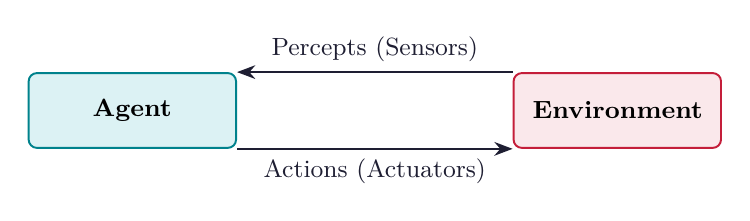
\begin{tikzpicture}[node distance=1.8cm, auto]
  \node [block] (agent) {\textbf{Agent}};
  \node [block, fill=hdrred, draw=myred, right=3.5cm of agent] (env) {\textbf{Environment}};
  
  \draw [arrow] (env.north west) -- node[above, font=\small] {Percepts (Sensors)} (agent.north east);
  \draw [arrow] (agent.south east) -- node[below, font=\small] {Actions (Actuators)} (env.south west);
\end{tikzpicture}
\end{tcolorbox}

\subsection{PEAS Specification}
To design an intelligent agent, we must explicitly define its \textbf{PEAS} properties:
\begin{itemize}[leftmargin=*, itemsep=3pt]
  \item \textbf{P --- Performance Measure:} Objective criteria evaluating the success of the agent's behavior.
  \item \textbf{E --- Environment:} External surroundings and domain in which the agent operates.
  \item \textbf{A --- Actuators:} Mechanisms through which the agent performs actions.
  \item \textbf{S --- Sensors:} Instruments through which the agent receives inputs/percepts.
\end{itemize}

\par\vspace{6pt}\noindent
{\renewcommand{\arraystretch}{1.4}%
\begin{tabularx}{\linewidth}{|B{2.8cm}|Y|Y|Y|Y|}
\hline
\textbf{Agent Type} & \textbf{Performance Measure} & \textbf{Environment} & \textbf{Actuators} & \textbf{Sensors} \\
\hline
Automated Taxi Driver & Safe, fast, legal, comfortable, max profit & Roads, traffic, pedestrians, weather & Steering, accelerator, brake, horn & Cameras, LiDAR, GPS, speedometer \\
\hline
Medical Diagnosis & Healthy patient, min cost, no lawsuits & Patient, hospital staff, laboratory & Screen display (reports, prescriptions) & Keyboard (symptoms, lab test results) \\
\hline
Vacuum Cleaner & Clean floor, min time, min electricity & Rooms, dirt, obstacles, carpet & Wheels, vacuum motor, brushes & Bump sensor, dirt detection sensor \\
\hline
\end{tabularx}}

\subsection{Concept of Rationality}
A \textbf{Rational Agent} is one that operates to choose actions that maximize its expected performance measure, given the evidence provided by the percept sequence and whatever built-in knowledge the agent possesses.

\begin{tcolorbox}[examplebox, title={Factors Determining Rationality}]
  Rationality depends on 4 parameters:
  \begin{enumerate}[leftmargin=*, noitemsep]
    \item The \textbf{Performance Measure} defining the success criterion.
    \item The agent's \textbf{Prior Knowledge} of the environment.
    \item The \textbf{Actions} that the agent can perform.
    \item The agent's \textbf{Percept Sequence} up to the present moment.
  \end{enumerate}
\end{tcolorbox}

% ===============================================================================
\section{Environment Properties and Agent Structures}
% ===============================================================================

\subsection{Classification of Environments}
\begin{itemize}[leftmargin=*, itemsep=4pt]
  \item \textbf{Fully Observable vs. Partially Observable:} An environment is fully observable if sensors give complete state access at any time (e.g., Chess vs. Poker / Medical Diagnosis).
  \item \textbf{Single-Agent vs. Multi-Agent:} Single-agent operates alone (Crossword); Multi-agent involves other agents (Chess, Taxi driving). Multi-agent can be competitive or cooperative.
  \item \textbf{Deterministic vs. Stochastic:} Deterministic if next state is completely determined by current state and action (Chess). Stochastic if uncertainty exists (Taxi driving, Ludo).
  \item \textbf{Episodic vs. Sequential:} Episodic means current decision does not affect future decisions (Image classification). Sequential means current actions affect future decisions (Chess).
  \item \textbf{Static vs. Dynamic:} Static environment does not change while agent is deliberating (Crossword). Dynamic environment changes continuously (Taxi driver). Semi-dynamic if environment doesn't change but agent score decreases with time (Timed Chess).
  \item \textbf{Discrete vs. Continuous:} Discrete has finite, distinct states and actions (Chess). Continuous has continuous parameters like speed, angle, temperature (Taxi driver).
  \item \textbf{Known vs. Unknown:} Known means environment laws/physics are given to the agent (Solitaire). Unknown means laws must be learned (New video game).
\end{itemize}

\subsection{Four Basic Agent Architectures}

\subsubsection{1. Simple Reflex Agent}
Selects actions based \textbf{only on the current percept}, ignoring percept history. Uses Condition-Action Rules (`IF condition THEN action`).

\begin{tcolorbox}[tikzbox, title={Simple Reflex Agent Architecture}]
\centering
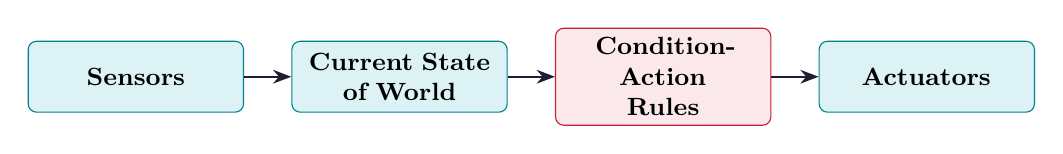
\begin{tikzpicture}[
  node distance=0.6cm, auto,
  sblock/.style={draw=myteal, fill=hdrteal, rectangle, rounded corners=3pt, align=center, font=\small\bfseries, minimum height=0.9cm, text width=2.5cm}
]
  \node [sblock] (sensor) {Sensors};
  \node [sblock, right=0.6cm of sensor] (state) {Current State\\of World};
  \node [sblock, fill=hdrred, draw=myred, right=0.6cm of state] (rule) {Condition-Action\\Rules};
  \node [sblock, right=0.6cm of rule] (act) {Actuators};
  
  \draw [arrow] (sensor) -- (state);
  \draw [arrow] (state) -- (rule);
  \draw [arrow] (rule) -- (act);
\end{tikzpicture}
\end{tcolorbox}

\subsubsection{2. Model-Based Reflex Agent}
Maintains an internal \textbf{state} tracking aspects of the environment not currently visible. Requires knowledge of how the world evolves and how agent actions affect the world.

\subsubsection{3. Goal-Based Agent}
Combines state information with \textbf{goal information} to choose actions that achieve the desired outcome. Uses search and planning.

\subsubsection{4. Utility-Based Agent}
Uses a \textbf{utility function} mapping a state onto a real number to measure happiness/desirability of states. Allows tradeoff choices under conflicting goals.

\newpage
\begin{center}
  {\large\bfseries\color{myred} Quick Revision --- Module 1}\\[3pt]
  {\small\color{mydark} Introduction to AI \& Intelligent Agents $|$ OE-EC804A}
\end{center}
\noindent{\color{myred}\rule{\linewidth}{1.2pt}}
\vspace{4pt}

\begin{tcolorbox}[formulabox, title={\textbf{Key Concepts and Metrics at a Glance}}]
\renewcommand{\arraystretch}{1.35}
\begin{tabularx}{\linewidth}{B{4.5cm} X}
Agent Function & $f: \mathcal{P}^* \to \mathcal{A}$ mapping percept histories to actions. \\[4pt]
PEAS Specification & Performance Measure, Environment, Actuators, Sensors. \\[4pt]
Rationality & Maximizes expected performance based on percept sequence \& prior knowledge. \\[4pt]
Turing Test & 6 core capabilities: NLP, Knowledge Rep, Reasoning, ML, Vision, Robotics. \\[4pt]
Environment Dimensions & 7 attributes: Observable, Multi-agent, Deterministic, Sequential, Static, Discrete, Known. \\
\end{tabularx}
\end{tcolorbox}

\begin{tcolorbox}[defbox, title={\textbf{One-Line Definitions}}]
  \begin{itemize}[leftmargin=*, noitemsep]
    \item \textbf{Rational Agent:} An agent that acts to achieve the best expected performance outcome.
    \item \textbf{PEAS:} Formal framework defining an agent's task environment.
    \item \textbf{Simple Reflex Agent:} Operates strictly on current percept using Condition-Action rules.
    \item \textbf{Model-Based Agent:} Maintains internal state to handle partial observability.
    \item \textbf{Utility-Based Agent:} Evaluates action choices using a quantitative utility function.
  \end{itemize}
\end{tcolorbox}

\begin{tcolorbox}[exambox, title={\textbf{Frequently Asked / Viva Questions}}]
  \begin{enumerate}[topsep=0pt, label=\textbf{Q\arabic*.}, itemsep=5pt]
    \item \Q{Define Artificial Intelligence. List the four perspectives of AI definitions.}
    AI is the field of computer science creating systems capable of human-like intelligence. The 4 perspectives are: Thinking Humanly, Acting Humanly (Turing Test), Thinking Rationally (Logic), and Acting Rationally (Rational Agents).

    \item \Q{What is the Turing Test? What capabilities are required to pass it?}
    Proposed by Alan Turing in 1950, it tests if a machine can imitate human conversation convincingly. Required capabilities: NLP, Knowledge Representation, Automated Reasoning, Machine Learning, Computer Vision, and Robotics.

    \item \Q{What is an Agent and Agent Function?}
    An agent perceives environment via sensors and acts via actuators. Agent function $f: \mathcal{P}^* \to \mathcal{A}$ maps percept histories to actions.

    \item \Q{Explain the PEAS framework with an example.}
    PEAS stands for Performance, Environment, Actuators, Sensors. For automated taxi: P=Safety/Speed, E=Roads/Traffic, A=Steering/Brake, S=Cameras/Radar.

    \item \Q{Distinguish between Rationality and Omniscience.}
    Rationality maximizes expected performance based on available percepts. Omniscience knows actual outcome in advance. Rationality is feasible; omniscience is impossible in uncertain environments.

    \item \Q{Differentiate between Deterministic and Stochastic environments.}
    Deterministic: Next state is completely fixed by current state and action. Stochastic: Next state involves probability and randomness.

    \item \Q{What is a Simple Reflex Agent?}
    An agent that acts based strictly on the current percept using IF-THEN condition-action rules without memory.

    \item \Q{Why does a Model-Based Reflex Agent need internal state?}
    To handle partially observable environments by tracking unobserved aspects of the world over time.

    \item \Q{Compare Goal-Based vs Utility-Based Agents.}
    Goal-based agents focus on reaching a target state (binary success). Utility-based agents evaluate degree of desirability (continuous score/utility) to make optimal tradeoffs.

    \item \Q{Explain Episodic vs Sequential environments.}
    Episodic: Each episode is independent; action choice does not impact future states. Sequential: Actions impact all future states (e.g. Chess).
  \end{enumerate}
\end{tcolorbox}


% -- Module 2 -----------------------------------------------------------------
\modulestart{2}{Problem-Solving Agents \& Problem Formulation}

\section{Problem-Solving Agents \& Problem Formulation}
% ===============================================================================

A \textbf{Problem-Solving Agent} is a goal-based agent that decides what to do by finding sequences of actions that lead to desirable states.

\begin{tcolorbox}[defbox, title={Definition of a Problem}]
  A \textbf{Problem} is formally defined by 5 components:
  \begin{enumerate}[leftmargin=*, noitemsep]
    \item \textbf{Initial State:} $s_0 \in S$, the state where the agent begins.
    \item \textbf{Actions:} $Actions(s)$, the set of valid actions available in state $s$.
    \item \textbf{Transition Model:} $Result(s, a)$, returns the outcome state resulting from taking action $a$ in state $s$.
    \item \textbf{Goal Test:} Function determining whether a given state is a goal state.
    \item \textbf{Path Cost:} $c(s, a, s')$, numeric cost assigned to taking step $a$ from $s$ to $s'$.
  \end{enumerate}
\end{tcolorbox}

\subsection{State Space and Search Trees}
\begin{itemize}[leftmargin=*, itemsep=3pt]
  \item \textbf{State Space:} The set of all reachable states from the initial state via any sequence of actions.
  \item \textbf{Search Space / Tree:} A tree generated by the search algorithm where the root is the initial state and child nodes correspond to actions.
  \item \textbf{Branching Factor ($b$):} Maximum number of successors (children) of any node.
  \item \textbf{Depth ($d$):} Depth of the shallowest goal node.
  \item \textbf{Maximum Depth ($m$):} Maximum length of any path in the state space.
\end{itemize}

\subsection{Evaluation Criteria for Search Algorithms}
Search algorithms are evaluated based on four fundamental metrics:
\begin{enumerate}[leftmargin=*, itemsep=3pt]
  \item \textbf{Completeness:} Is the algorithm guaranteed to find a solution if one exists?
  \item \textbf{Time Complexity:} How long (how many nodes generated) does it take to find a solution?
  \item \textbf{Space Complexity:} How much memory is needed to perform the search?
  \item \textbf{Optimality:} Does the strategy find the lowest path cost solution?
\end{enumerate}

% ===============================================================================
\section{Uninformed Search Strategies}
% ===============================================================================

Uninformed search (blind search) strategies have no additional information about states beyond that provided in the problem definition.

\begin{tcolorbox}[tikzbox, title={Sample Search Tree Topology}]
\centering
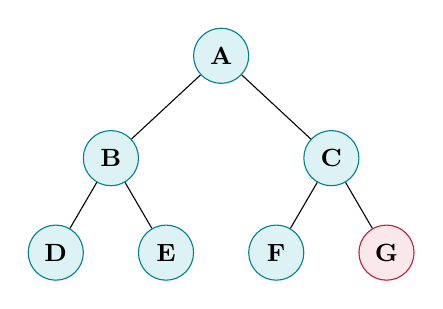
\begin{tikzpicture}[
  level 1/.style={sibling distance=2.8cm, level distance=1.3cm},
  level 2/.style={sibling distance=1.4cm, level distance=1.2cm},
  every node/.style={circle, draw=myteal, fill=hdrteal, inner sep=2pt, font=\small\bfseries, minimum size=0.7cm}
]
  \node {A}
    child {node {B}
      child {node {D}}
      child {node {E}}
    }
    child {node {C}
      child {node {F}}
      child [style={every node/.append style={draw=myred, fill=hdrred}}] {node {G}}
    };
\end{tikzpicture}
\end{tcolorbox}

\subsection{1. Breadth-First Search (BFS)}
\begin{itemize}[leftmargin=*, itemsep=3pt]
  \item \textbf{Mechanism:} Expands the root node first, then expands all successors of the root, then their successors. Implemented using a \textbf{FIFO (Queue)} frontier.
  \item \textbf{Completeness:} Complete (if branching factor $b$ is finite).
  \item \textbf{Time Complexity:} $O(b^d)$
  \item \textbf{Space Complexity:} $O(b^d)$ (all nodes kept in memory).
  \item \textbf{Optimality:} Optimal if step costs are uniform (equal to 1).
\end{itemize}

\subsection{2. Depth-First Search (DFS)}
\begin{itemize}[leftmargin=*, itemsep=3pt]
  \item \textbf{Mechanism:} Expands the deepest node in the current frontier. Implemented using a \textbf{LIFO (Stack)} frontier.
  \item \textbf{Completeness:} Incomplete in infinite state spaces or graphs with loops.
  \item \textbf{Time Complexity:} $O(b^m)$
  \item \textbf{Space Complexity:} $O(b \cdot m)$ (linear memory overhead!).
  \item \textbf{Optimality:} Non-optimal (may find a deeper solution before a shallow one).
\end{itemize}

\subsection{3. Depth-Limited Search (DLS)}
\begin{itemize}[leftmargin=*, itemsep=3pt]
  \item \textbf{Mechanism:} DFS with a pre-determined depth limit $l$. Nodes at depth $l$ are treated as if they have no successors.
  \item \textbf{Completeness:} Incomplete if $l < d$.
  \item \textbf{Time Complexity:} $O(b^l)$
  \item \textbf{Space Complexity:} $O(b \cdot l)$
  \item \textbf{Optimality:} Non-optimal if $l > d$.
\end{itemize}

\subsection{4. Iterative Deepening DFS (IDDFS)}
\begin{itemize}[leftmargin=*, itemsep=3pt]
  \item \textbf{Mechanism:} Combines the benefits of BFS (completeness/optimality) and DFS (linear memory). It calls DLS repeatedly with increasing depth limits $l = 0, 1, 2, \dots$
  \item \textbf{Completeness:} Complete (if $b$ is finite).
  \item \textbf{Time Complexity:} $O(b^d)$
  \item \textbf{Space Complexity:} $O(b \cdot d)$ (Linear space!).
  \item \textbf{Optimality:} Optimal if step costs are equal.
\end{itemize}

\subsection{5. Bidirectional Search}
\begin{itemize}[leftmargin=*, itemsep=3pt]
  \item \textbf{Mechanism:} Runs two simultaneous searches: one forward from initial state and one backward from goal state. Stops when frontiers intersect.
  \item \textbf{Completeness:} Complete if $b$ is finite and both searches are BFS.
  \item \textbf{Time Complexity:} $O(b^{d/2})$
  \item \textbf{Space Complexity:} $O(b^{d/2})$
  \item \textbf{Optimality:} Optimal if step costs are uniform.
\end{itemize}

% ===============================================================================
\section{Comparison of Search Strategies}
% ===============================================================================

\par\vspace{6pt}\noindent
{\renewcommand{\arraystretch}{1.45}%
\begin{tabularx}{\linewidth}{|B{3.0cm}|Y|Y|Y|Y|}
\hline
\textbf{Criterion} & \textbf{BFS} & \textbf{DFS} & \textbf{IDDFS} & \textbf{Bidirectional} \\
\hline
Completeness & Yes (if $b<\infty$) & No & Yes (if $b<\infty$) & Yes (if $b<\infty$) \\
\hline
Time Complexity & $O(b^d)$ & $O(b^m)$ & $O(b^d)$ & $O(b^{d/2})$ \\
\hline
Space Complexity & $O(b^d)$ & $O(b \cdot m)$ & $O(b \cdot d)$ & $O(b^{d/2})$ \\
\hline
Optimality & Yes (cost = 1) & No & Yes (cost = 1) & Yes (cost = 1) \\
\hline
Frontier Data Struct & FIFO Queue & LIFO Stack & LIFO Stack (Iterative) & Two FIFO Queues \\
\hline
\end{tabularx}}

\newpage
\begin{center}
  {\large\bfseries\color{myred} Quick Revision --- Module 2}\\[3pt]
  {\small\color{mydark} Solving Problems by Searching (Uninformed Search) $|$ OE-EC804A}
\end{center}
\noindent{\color{myred}\rule{\linewidth}{1.2pt}}
\vspace{4pt}

\begin{tcolorbox}[formulabox, title={\textbf{Key Concepts and Metrics at a Glance}}]
\renewcommand{\arraystretch}{1.35}
\begin{tabularx}{\linewidth}{B{4.5cm} X}
BFS Complexity & Time: $O(b^d)$, Space: $O(b^d)$ \quad (FIFO Queue, Complete, Optimal for step cost = 1) \\[4pt]
DFS Complexity & Time: $O(b^m)$, Space: $O(b \cdot m)$ \quad (LIFO Stack, Incomplete, Non-optimal) \\[4pt]
IDDFS Complexity & Time: $O(b^d)$, Space: $O(b \cdot d)$ \quad (Linear memory, Complete, Optimal) \\[4pt]
Bidirectional Search & Time: $O(b^{d/2})$, Space: $O(b^{d/2})$ \quad (Searches forward \& backward) \\[4pt]
Problem Components & Initial state $s_0$, Actions $Actions(s)$, Transition model $Result(s,a)$, Goal test, Path cost. \\
\end{tabularx}
\end{tcolorbox}

\begin{tcolorbox}[defbox, title={\textbf{One-Line Definitions}}]
  \begin{itemize}[leftmargin=*, noitemsep]
    \item \textbf{State Space:} Set of all valid states reachable from initial state.
    \item \textbf{Frontier:} Set of leaf nodes generated but not yet expanded.
    \item \textbf{Branching Factor ($b$):} Maximum number of successors for any node.
    \item \textbf{IDDFS:} Strategy running DLS with increasing limits $l=0,1,2,\dots$ combining BFS optimality with DFS space.
  \end{itemize}
\end{tcolorbox}

\begin{tcolorbox}[exambox, title={\textbf{Frequently Asked / Viva Questions}}]
  \begin{enumerate}[topsep=0pt, label=\textbf{Q\arabic*.}, itemsep=5pt]
    \item \Q{What are the 5 components of a formal problem definition?}
    Initial state, Actions, Transition model, Goal test, and Path cost.

    \item \Q{Compare BFS and DFS in terms of space complexity.}
    BFS requires $O(b^d)$ space (exponential), whereas DFS requires only $O(b \cdot m)$ space (linear).

    \item \Q{Why is IDDFS preferred over BFS for large state spaces?}
    IDDFS is complete and optimal like BFS, but uses linear space $O(b \cdot d)$ instead of exponential space $O(b^d)$.

    \item \Q{Why does node regeneration in IDDFS not incur high overhead?}
    Most nodes in a search tree are at the bottom level ($d$). Nodes at level $d$ are generated 1 time, level $d-1$ twice, etc., so total nodes generated $\approx \frac{b}{b-1} b^d$, which is asymptotically $O(b^d)$.

    \item \Q{What is the frontier in search algorithms?}
    The data structure (queue/stack) containing generated nodes that have not yet been expanded.

    \item \Q{When is BFS optimal?}
    BFS is optimal when all step costs are equal (uniform path cost).

    \item \Q{Explain the time and space complexity of Bidirectional Search.}
    Time and space complexities are both $O(b^{d/2})$ because two searches meet in the middle.

    \item \Q{What is Depth-Limited Search and why is it used?}
    DFS restricted to depth limit $l$. It prevents DFS from getting stuck in infinite paths.

    \item \Q{What is a Graph Search vs Tree Search?}
    Graph search maintains an `explored set` to avoid repeating states in looped graphs. Tree search does not.

    \item \Q{Define Completeness and Optimality.}
    Completeness: Guaranteed to find a solution if one exists. Optimality: Guaranteed to find the lowest-cost solution.
  \end{enumerate}
\end{tcolorbox}


% -- Module 3 -----------------------------------------------------------------
\modulestart{3}{Informed (Heuristic) Search Strategies}

\section{Informed (Heuristic) Search Strategies}
% ===============================================================================

Informed search strategies use domain-specific knowledge provided by a \textbf{Heuristic Function} $h(n)$ to guide the search towards goal states more efficiently.

\begin{tcolorbox}[defbox, title={Definition of a Heuristic Function}]
  A \textbf{Heuristic Function} $h(n)$ estimates the cost of the cheapest path from state $n$ to a goal state. For any goal state $g$, $h(g) = 0$.
\end{tcolorbox}

\subsection{1. Greedy Best-First Search}
\begin{itemize}[leftmargin=*, itemsep=3pt]
  \item \textbf{Evaluation Function:} $f(n) = h(n)$.
  \item Expands the node that appears to be closest to the goal.
  \item \textbf{Properties:} Incomplete in looped graphs; non-optimal. Time and Space complexity $O(b^m)$ worst-case.
\end{itemize}

\subsection{2. A* Search Algorithm}
A* combines the cost-so-far $g(n)$ and estimated remaining cost $h(n)$.

\begin{tcolorbox}[formulabox, title={A* Evaluation Function}]
  \begin{equation}
    f(n) = g(n) + h(n)
  \end{equation}
  where:
  \begin{itemize}[leftmargin=*, noitemsep]
    \item $g(n)$: Exact path cost from initial state to node $n$.
    \item $h(n)$: Estimated cost from node $n$ to goal state.
    \item $f(n)$: Estimated total cost of path through $n$ to goal.
  \end{itemize}
\end{tcolorbox}

\subsection{Conditions for A* Optimality}
\begin{enumerate}[leftmargin=*, itemsep=4pt]
  \item \textbf{Admissibility (Tree Search Optimality):}
    A heuristic $h(n)$ is admissible if it \textbf{never overestimates} the true cost to reach the goal:
    \begin{equation}
      h(n) \le h^*(n) \quad \forall n
    \end{equation}
    where $h^*(n)$ is the true minimum cost from $n$ to goal.
  
  \item \textbf{Monotonicity / Consistency (Graph Search Optimality):}
    A heuristic $h(n)$ is consistent if for every node $n$ and successor $n'$ generated by action $a$:
    \begin{equation}
      h(n) \le c(n, a, n') + h(n')
    \end{equation}
    This satisfies the triangle inequality and guarantees $f(n)$ is non-decreasing along any path.
\end{enumerate}

\subsection{On-line Search Agents and Unknown Environments}
Unlike offline search algorithms (which compute a complete solution path before taking their first action), an \textbf{On-line Search Agent} interleaves computation and action: it acts, observes the new state, and decides its next move.

\begin{tcolorbox}[defbox, title={On-line Search Agent}]
  An \textbf{On-line Search Agent} operates in unknown or dynamic environments by exploring state space physically. It computes an action, executes it in the environment, senses the resulting state $s'$, and updates its internal map.
\end{tcolorbox}

\begin{itemize}[leftmargin=*, itemsep=3pt]
  \item \textbf{Offline vs. On-line Search:} Offline agents compute the full path in a simulator before moving. On-line agents move in the physical world to discover state transitions and costs.
  \item \textbf{Competitive Ratio:} Evaluates on-line search performance by comparing actual path cost incurred to the optimal path cost if the environment were known in advance.
  \item \textbf{LRTA* (Learning Real-Time A*):} An on-line search algorithm that updates heuristic estimates $H(s)$ of visited states based on neighbor cost:
    \begin{equation}
      H(s) \leftarrow \min_{a \in Actions(s)} \left[ c(s, a, s') + H(s') \right]
    \end{equation}
\end{itemize}

% ===============================================================================
\section{Constraint Satisfaction Problems (CSPs)}
% ===============================================================================

\begin{tcolorbox}[defbox, title={Definition of a CSP}]
  A \textbf{Constraint Satisfaction Problem (CSP)} is defined by a triple $(X, D, C)$:
  \begin{itemize}[leftmargin=*, noitemsep]
    \item $X = \{X_1, X_2, \dots, X_n\}$: Set of variables.
    \item $D = \{D_1, D_2, \dots, D_n\}$: Set of domains (possible values for each variable).
    \item $C = \{C_1, C_2, \dots, C_m\}$: Set of constraints specifying allowable value combinations.
  \end{itemize}
\end{tcolorbox}

\begin{tcolorbox}[tikzbox, title={Constraint Graph Representation (Map Coloring Example)}]
\centering
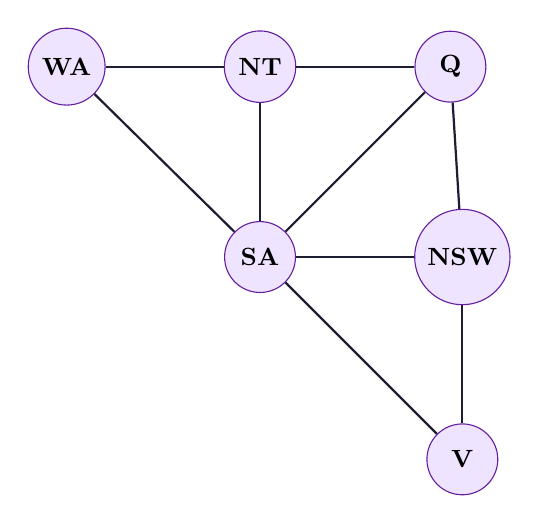
\begin{tikzpicture}[node distance=1.5cm, auto]
  \node [cnode] (wa) {WA};
  \node [cnode, right=of wa] (nt) {NT};
  \node [cnode, right=of nt] (q) {Q};
  \node [cnode, below=of nt] (sa) {SA};
  \node [cnode, right=of sa] (nsw) {NSW};
  \node [cnode, below=of nsw] (v) {V};

  \draw [line] (wa) -- (nt);
  \draw [line] (wa) -- (sa);
  \draw [line] (nt) -- (sa);
  \draw [line] (nt) -- (q);
  \draw [line] (q) -- (sa);
  \draw [line] (q) -- (nsw);
  \draw [line] (sa) -- (nsw);
  \draw [line] (sa) -- (v);
  \draw [line] (nsw) -- (v);
\end{tikzpicture}
\end{tcolorbox}

\subsection{Backtracking Search for CSPs}
Backtracking search is a depth-first search that chooses values for one variable at a time and backtracks when a variable has no legal values left.

\begin{tcolorbox}[examplebox, title={Heuristics for CSP Backtracking}]
  \begin{enumerate}[leftmargin=*, noitemsep]
    \item \textbf{Minimum Remaining Values (MRV):} Choose variable with fewest legal values remaining ("fail-first" heuristic).
    \item \textbf{Degree Heuristic:} Choose variable involved in largest number of constraints on unassigned variables.
    \item \textbf{Least Constraining Value (LCV):} Choose value that rules out fewest choices for neighboring variables.
  \end{enumerate}
\end{tcolorbox}

\subsection{Constraint Propagation \& AC-3 Algorithm}
Constraint propagation enforces local consistency to prune search spaces early.

\begin{itemize}[leftmargin=*, itemsep=3pt]
  \item \textbf{Forward Checking:} When variable $X$ is assigned, remove inconsistent values from domains of unassigned neighbors.
  \item \textbf{Arc Consistency (AC-3):} Arc $X_i \to X_j$ is consistent if for every value $x \in D_i$, there exists an allowed value $y \in D_j$.
\end{itemize}

\subsection{Local Search for CSPs (Min-Conflicts Algorithm)}
Unlike backtracking search which operates on partial assignments, local search algorithms for CSPs use a \textbf{complete-state formulation}: every variable is initially assigned a value (even if constraints are violated).

\begin{tcolorbox}[defbox, title={Min-Conflicts Heuristic}]
  In each iteration, \textbf{Min-Conflicts} randomly selects a conflicted variable $X_i$ and reassigns it the value $v \in D_i$ that minimizes the total number of constraint violations across the CSP.
\end{tcolorbox}

\begin{itemize}[leftmargin=*, itemsep=3pt]
  \item \textbf{Algorithm Mechanism:} Start with a complete assignment $\to$ pick a conflicted variable $X$ at random $\to$ set $X$ to value minimizing constraint violations $\to$ repeat until solution or step limit.
  \item \textbf{Performance:} Solves $N$-Queens for $N = 1,000,000$ in seconds; space complexity is $O(n)$ (linear).
  \item \textbf{Escaping Local Minima:} Uses random walks, simulated annealing, or random restarts to escape plateau states.
\end{itemize}

\newpage
\begin{center}
  {\large\bfseries\color{myred} Quick Revision --- Module 3}\\[3pt]
  {\small\color{mydark} Informed Search \& Constraint Satisfaction Problems $|$ OE-EC804A}
\end{center}
\noindent{\color{myred}\rule{\linewidth}{1.2pt}}
\vspace{4pt}

\begin{tcolorbox}[formulabox, title={\textbf{Key Concepts and Metrics at a Glance}}]
\renewcommand{\arraystretch}{1.35}
\begin{tabularx}{\linewidth}{B{4.5cm} X}
A* Evaluation Function & $f(n) = g(n) + h(n)$ \quad ($g(n)$ cost-so-far, $h(n)$ estimated remaining cost) \\[4pt]
Admissibility Condition & $h(n) \le h^*(n)$ \quad (Heuristic never overestimates true cost to goal) \\[4pt]
Consistency Condition & $h(n) \le c(n, a, n') + h(n')$ \quad (Satisfies triangle inequality along edges) \\[4pt]
CSP Formalization & Triple $(X, D, C)$ of Variables, Domains, and Constraints \\[4pt]
Min-Conflicts Heuristic & Local search reassigning conflicted variable value to minimize violations. \\
\end{tabularx}
\end{tcolorbox}

\begin{tcolorbox}[defbox, title={\textbf{One-Line Definitions}}]
  \begin{itemize}[leftmargin=*, noitemsep]
    \item \textbf{Admissible Heuristic:} A heuristic that never overestimates the actual cost to reach goal.
    \item \textbf{Consistent Heuristic:} A heuristic obeying triangle inequality along graph edges.
    \item \textbf{Arc Consistency (AC-3):} State where every value in a variable domain has a valid partner in neighbor domains.
    \item \textbf{MRV Heuristic:} Chooses the variable with the fewest remaining legal domain choices.
  \end{itemize}
\end{tcolorbox}

\begin{tcolorbox}[exambox, title={\textbf{Frequently Asked / Viva Questions}}]
  \begin{enumerate}[topsep=0pt, label=\textbf{Q\arabic*.}, itemsep=5pt]
    \item \Q{Define A* search. What is its evaluation function?}
    A* evaluates nodes using $f(n) = g(n) + h(n)$, combining cost-so-far $g(n)$ and heuristic estimate $h(n)$.

    \item \Q{What is an Admissible Heuristic?}
    A heuristic $h(n)$ that never overestimates true cost to goal ($h(n) \le h^*(n)$).

    \item \Q{Differentiate between Admissibility and Consistency.}
    Admissibility guarantees optimality for tree search. Consistency ($h(n) \le c(n,a,n') + h(n')$) guarantees $f(n)$ is non-decreasing, ensuring optimality for graph search without re-opening nodes.

    \item \Q{Define CSP formally.}
    A triple $(X, D, C)$ where $X$ is set of variables, $D$ set of domains, and $C$ set of constraints.

    \item \Q{Explain the MRV heuristic in CSPs.}
    Minimum Remaining Values heuristic chooses the variable with fewest valid remaining choices, aiming to fail early.

    \item \Q{What is Forward Checking?}
    In CSP search, whenever variable $X$ is assigned, any inconsistent values are pruned from neighboring unassigned variables.

    \item \Q{What is the AC-3 algorithm?}
    An algorithm that enforces arc consistency across all variable pairs in a CSP constraint graph.

    \item \Q{Compare Greedy Best-First Search and A* Search.}
    Greedy uses $f(n) = h(n)$ (fast, non-optimal). A* uses $f(n) = g(n) + h(n)$ (optimal if $h$ is admissible).

    \item \Q{What is Manhattan Distance heuristic in 8-puzzle?}
    Sum of absolute differences in horizontal and vertical coordinates of tiles from goal positions.

    \item \Q{Why is LCV used for value selection in CSPs?}
    Least Constraining Value maximizes flexibility for remaining variables, leaving maximal choices open.
  \end{enumerate}
\end{tcolorbox}


% -- Module 4 -----------------------------------------------------------------
\modulestart{4}{Games as Search Problems}

\section{Games as Search Problems}
% ===============================================================================

In AI, competitive multi-agent environments are modeled as \textbf{Adversarial Search Problems} or \textbf{Games}.

\begin{tcolorbox}[defbox, title={Formal Definition of a Game}]
  A 2-player deterministic zero-sum game is defined by:
  \begin{enumerate}[leftmargin=*, noitemsep]
    \item \textbf{$S_0$:} Initial state of the game board.
    \item \textbf{$Player(s)$:} Defines whose turn it is to move in state $s$.
    \item \textbf{$Actions(s)$:} Set of legal moves available in state $s$.
    \item \textbf{$Result(s, a)$:} Transition model returning state outcome of move $a$ in state $s$.
    \item \textbf{$Terminal\text{-}Test(s)$:} True if game is over; false otherwise.
    \item \textbf{$Utility(s, p)$:} Final numeric value for game outcome state $s$ for player $p$.
  \end{enumerate}
\end{tcolorbox}

\subsection{Zero-Sum Property}
In a \textbf{Zero-Sum Game}, the total utility across players is constant. For 2 players (MAX and MIN):
\begin{equation}
  Utility_{MAX}(s) + Utility_{MIN}(s) = 0
\end{equation}
MAX attempts to maximize the utility, while MIN attempts to minimize it.

% ===============================================================================
\section{The Minimax Algorithm}
% ===============================================================================

\begin{tcolorbox}[formulabox, title={Minimax Value Definition}]
  \begin{equation}
    Minimax(s) = \begin{cases}
      Utility(s) & \text{if } Terminal\text{-}Test(s) \\
      \max_{a \in Actions(s)} Minimax(Result(s, a)) & \text{if } Player(s) = MAX \\
      \min_{a \in Actions(s)} Minimax(Result(s, a)) & \text{if } Player(s) = MIN
    \end{cases}
  \end{equation}
\end{tcolorbox}

\begin{tcolorbox}[tikzbox, title={Minimax Game Tree Visualization}]
\centering
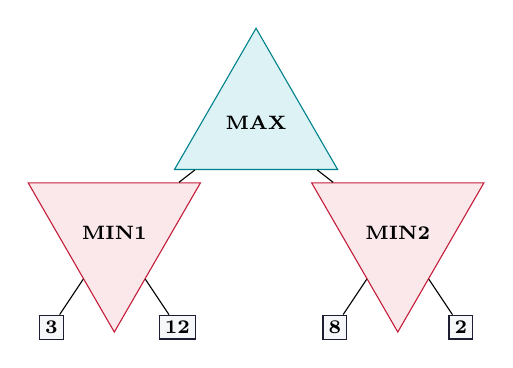
\begin{tikzpicture}[
  level 1/.style={sibling distance=3.6cm, level distance=1.4cm},
  level 2/.style={sibling distance=1.6cm, level distance=1.2cm}
]
  \node [maxnode] {MAX}
    child {node [minnode] {MIN1}
      child {node [leaf] {3}}
      child {node [leaf] {12}}
    }
    child {node [minnode] {MIN2}
      child {node [leaf] {8}}
      child {node [leaf] {2}}
    };
\end{tikzpicture}
\end{tcolorbox}

\subsection{Properties of Minimax}
\begin{itemize}[leftmargin=*, itemsep=3pt]
  \item \textbf{Completeness:} Complete if tree is finite.
  \item \textbf{Optimality:} Optimal against an optimal opponent.
  \item \textbf{Time Complexity:} $O(b^m)$ (explores all tree nodes).
  \item \textbf{Space Complexity:} $O(b \cdot m)$ (depth-first traversal).
\end{itemize}

% ===============================================================================
\section{Alpha-Beta Pruning}
% ===============================================================================

Alpha-Beta pruning removes branches of the game tree that cannot influence the final decision, reducing search time without altering the optimal choice.

\begin{tcolorbox}[defbox, title={Definition of Alpha ($\alpha$) and Beta ($\beta$)}]
  \begin{itemize}[leftmargin=*, noitemsep]
    \item \textbf{$\alpha$ (Alpha):} Highest-value choice found so far along the path for MAX. (Initial value: $-\infty$).
    \item \textbf{$\beta$ (Beta):} Lowest-value choice found so far along the path for MIN. (Initial value: $+\infty$).
  \end{itemize}
\end{tcolorbox}

\begin{tcolorbox}[formulabox, title={Alpha-Beta Pruning Condition}]
  Prune remaining children of node $n$ if:
  \begin{equation}
    \alpha \ge \beta
  \end{equation}
\end{tcolorbox}

\subsection{Effectiveness of Alpha-Beta Pruning}
\begin{itemize}[leftmargin=*, itemsep=3pt]
  \item \textbf{Worst-Case Complexity:} $O(b^m)$ (no pruning occurs if worst moves evaluated first).
  \item \textbf{Optimal Move Ordering Complexity:} $O(b^{m/2})$
  \item With optimal move ordering, Alpha-Beta doubles the solvable search depth!
\end{itemize}

% ===============================================================================
\section{Imperfect Real-Time Decisions}
% ===============================================================================
In real games (Chess, Go), searching to terminal leaves is computationally impossible. We replace terminal tests with \textbf{Cutoff Tests} and terminal utility with \textbf{Evaluation Functions} $Eval(s)$.

\begin{tcolorbox}[examplebox, title={Requirements for Evaluation Functions}]
  \begin{enumerate}[leftmargin=*, noitemsep]
    \item Must rank terminal states in same order as true utility.
    \item Computation must be fast.
    \item Must correlate strongly with win probabilities (e.g., weighted sum of material values in Chess).
  \end{enumerate}
\end{tcolorbox}

\newpage
\begin{center}
  {\large\bfseries\color{myred} Quick Revision --- Module 4}\\[3pt]
  {\small\color{mydark} Adversarial Search \& Game Playing $|$ OE-EC804A}
\end{center}
\noindent{\color{myred}\rule{\linewidth}{1.2pt}}
\vspace{4pt}

\begin{tcolorbox}[formulabox, title={\textbf{Key Concepts and Metrics at a Glance}}]
\renewcommand{\arraystretch}{1.35}
\begin{tabularx}{\linewidth}{B{4.5cm} X}
Minimax Decision & $MAX = \max_{a} Minimax(Result(s,a))$, $MIN = \min_{a} Minimax(Result(s,a))$ \\[4pt]
$\alpha$-$\beta$ Pruning Condition & Prune remaining subtree whenever $\alpha \ge \beta$ \\[4pt]
Optimal Alpha-Beta Time & $O(b^{m/2})$ \quad (Doubles solvable search depth compared to $O(b^m)$) \\[4pt]
Evaluation Function & $Eval(s) = w_1 f_1(s) + w_2 f_2(s) + \dots + w_n f_n(s)$ \quad (Estimates utility at cutoff) \\[4pt]
Zero-Sum Property & $Utility_{MAX}(s) + Utility_{MIN}(s) = 0$ \quad (Constant total utility) \\
\end{tabularx}
\end{tcolorbox}

\begin{tcolorbox}[defbox, title={\textbf{One-Line Definitions}}]
  \begin{itemize}[leftmargin=*, noitemsep]
    \item \textbf{Zero-Sum Game:} Game where total utility across all players sums to zero.
    \item \textbf{Alpha ($\alpha$):} Best (highest) utility value MAX is guaranteed along path.
    \item \textbf{Beta ($\beta$):} Best (lowest) utility value MIN is guaranteed along path.
    \item \textbf{Horizon Effect:} Issue where inevitable bad event is pushed beyond search cutoff depth.
  \end{itemize}
\end{tcolorbox}

\begin{tcolorbox}[exambox, title={\textbf{Frequently Asked / Viva Questions}}]
  \begin{enumerate}[topsep=0pt, label=\textbf{Q\arabic*.}, itemsep=5pt]
    \item \Q{Define a Zero-Sum Game.}
    A game where one player's gain is exactly equal to the other player's loss ($Util_{MAX} + Util_{MIN} = 0$).

    \item \Q{What is the Minimax algorithm?}
    A recursive algorithm for calculating optimal moves in 2-player zero-sum games by maximizing MAX's payoff assuming MIN minimizes it.

    \item \Q{Explain Alpha ($\alpha$) and Beta ($\beta$) parameters.}
    $\alpha$: Best value for MAX found so far. $\beta$: Best value for MIN found so far.

    \item \Q{What is the condition for Alpha-Beta pruning?}
    Branch is pruned when $\alpha \ge \beta$.

    \item \Q{Does Alpha-Beta pruning change the final outcome of Minimax?}
    No, it produces the exact same decision as Minimax while pruning irrelevant branches.

    \item \Q{What is the time complexity of Alpha-Beta with perfect move ordering?}
    $O(b^{m/2})$, which doubles the effective search depth compared to standard Minimax ($O(b^m)$).

    \item \Q{Why are evaluation functions needed in game playing?}
    Because full game trees are too deep to search to terminal states within time limits.

    \item \Q{What is the Horizon Effect?}
    When search depth limit conceals an unavoidable penalty by delaying it past the cutoff.

    \item \Q{Compare Minimax vs Alpha-Beta Pruning.}
    Minimax evaluates all $O(b^m)$ nodes; Alpha-Beta prunes provably suboptimal branches reducing nodes to $O(b^{m/2})$.

    \item \Q{What is Quiescence Search?}
    Search expanded past cutoff depth in non-quiescent (unstable) states to prevent misleading evaluation scores.
  \end{enumerate}
\end{tcolorbox}


% -- Module 5 -----------------------------------------------------------------
\modulestart{5}{Knowledge-Based Agents \& Wumpus World}

\section{Knowledge-Based Agents \& Wumpus World}
% ===============================================================================

\begin{tcolorbox}[defbox, title={Definition of a Knowledge-Based Agent}]
  A \textbf{Knowledge-Based Agent} maintains an internal \textbf{Knowledge Base (KB)} expressed in a formal representation language. It operates by maintaining sentences in its KB, inserting new percepts via \texttt{TELL}, and deriving actions via \texttt{ASK}.
\end{tcolorbox}

\begin{tcolorbox}[formulabox, title={Core Operations of KB Agent}]
  \begin{itemize}[leftmargin=*, noitemsep]
    \item \texttt{TELL(KB, sentence)}: Adds new knowledge or percept to KB.
    \item \texttt{ASK(KB, query)}: Queries KB to infer whether query logically follows from KB.
  \end{itemize}
\end{tcolorbox}

\subsection{The Wumpus World Environment}
The \textbf{Wumpus World} is a benchmark domain for logical reasoning.
\begin{itemize}[leftmargin=*, itemsep=3pt]
  \item $4 \times 4$ grid of rooms containing a Wumpus, Pits, and Gold.
  \item \textbf{Percepts:} $[Stench, Breeze, Glitter, Bump, Scream]$.
  \item \textbf{Rules:} Rooms adjacent to Wumpus have $Stench$. Rooms adjacent to Pits have $Breeze$. Room containing Gold has $Glitter$.
\end{itemize}

\begin{tcolorbox}[tikzbox, title={Wumpus World Grid Environment ($4 \times 4$)}]
\centering
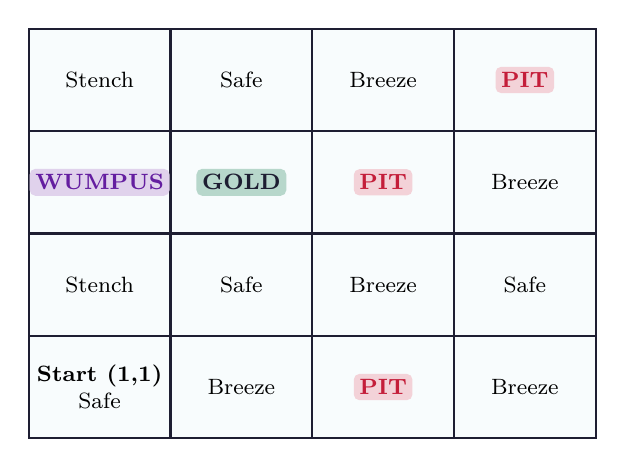
\begin{tikzpicture}[x=1.8cm, y=1.3cm]
  \draw[line, fill=hdrteal!20] (0,0) rectangle (4,4);
  \draw[line, step=1] (0,0) grid (4,4);
  
  % Row 1 (y=0.5)
  \node[align=center, font=\footnotesize] at (0.5,0.5) {\textbf{Start (1,1)}\\Safe};
  \node[align=center, font=\footnotesize] at (1.5,0.5) {Breeze};
  \node[align=center, font=\footnotesize, fill=myred!20, inner sep=2pt, rounded corners=2pt] at (2.5,0.5) {\textbf{\color{myred}PIT}};
  \node[align=center, font=\footnotesize] at (3.5,0.5) {Breeze};
  
  % Row 2 (y=1.5)
  \node[align=center, font=\footnotesize] at (0.5,1.5) {Stench};
  \node[align=center, font=\footnotesize] at (1.5,1.5) {Safe};
  \node[align=center, font=\footnotesize] at (2.5,1.5) {Breeze};
  \node[align=center, font=\footnotesize] at (3.5,1.5) {Safe};
  
  % Row 3 (y=2.5)
  \node[align=center, font=\footnotesize, fill=mypurple!20, inner sep=2pt, rounded corners=2pt] at (0.5,2.5) {\textbf{\color{mypurple}WUMPUS}};
  \node[align=center, font=\footnotesize, fill=mygreen!30, inner sep=2pt, rounded corners=2pt] at (1.5,2.5) {\textbf{\color{mydark}GOLD}};
  \node[align=center, font=\footnotesize, fill=myred!20, inner sep=2pt, rounded corners=2pt] at (2.5,2.5) {\textbf{\color{myred}PIT}};
  \node[align=center, font=\footnotesize] at (3.5,2.5) {Breeze};
  
  % Row 4 (y=3.5)
  \node[align=center, font=\footnotesize] at (0.5,3.5) {Stench};
  \node[align=center, font=\footnotesize] at (1.5,3.5) {Safe};
  \node[align=center, font=\footnotesize] at (2.5,3.5) {Breeze};
  \node[align=center, font=\footnotesize, fill=myred!20, inner sep=2pt, rounded corners=2pt] at (3.5,3.5) {\textbf{\color{myred}PIT}};
\end{tikzpicture}
\end{tcolorbox}

% ===============================================================================
\section{Propositional Logic}
% ===============================================================================

Propositional logic represents facts using proposition symbols ($P, Q, R$).

\begin{tcolorbox}[defbox, title={Logical Entailment}]
  Sentence $\alpha$ \textbf{entails} sentence $\beta$ ($\alpha \models \beta$) if and only if in every model in which $\alpha$ is true, $\beta$ is also true.
\end{tcolorbox}

\subsection{Logical Equivalences}
\par\vspace{6pt}\noindent
{\renewcommand{\arraystretch}{1.4}%
\begin{tabularx}{\linewidth}{|B{3.5cm}|Y|}
\hline
\textbf{Equivalence Law} & \textbf{Formula} \\
\hline
Implication Elimination & $\alpha \implies \beta \equiv \neg \alpha \lor \beta$ \\
\hline
Biconditional Elimination & $\alpha \iff \beta \equiv (\alpha \implies \beta) \land (\beta \implies \alpha)$ \\
\hline
De Morgan's Laws & $\neg(\alpha \land \beta) \equiv \neg \alpha \lor \neg \beta \quad ; \quad \neg(\alpha \lor \beta) \equiv \neg \alpha \land \neg \beta$ \\
\hline
Distributivity & $\alpha \land (\beta \lor \gamma) \equiv (\alpha \land \beta) \lor (\alpha \land \gamma)$ \\
\hline
\end{tabularx}}

% ===============================================================================
\section{Inference \& Resolution in Propositional Logic}
% ===============================================================================

\subsection{Resolution Rule}
Unit Resolution rule states that:
\begin{equation}
  \frac{l_1 \lor l_2 \lor \dots \lor l_k, \quad \neg l_i}{l_1 \lor \dots \lor l_{i-1} \lor l_{i+1} \lor \dots \lor l_k}
\end{equation}

Resolution Refutation proves $KB \models \alpha$ by showing that $KB \land \neg \alpha$ is \textbf{unsatisfiable}.

\subsection{Conjunctive Normal Form (CNF) Conversion Steps}
\begin{enumerate}[leftmargin=*, itemsep=3pt]
  \item Eliminate $\iff$ replacing $\alpha \iff \beta$ with $(\alpha \implies \beta) \land (\beta \implies \alpha)$.
  \item Eliminate $\implies$ replacing $\alpha \implies \beta$ with $\neg \alpha \lor \beta$.
  \item Move $\neg$ inwards using De Morgan's laws ($\neg(\alpha \lor \beta) \equiv \neg \alpha \land \neg \beta$).
  \item Distribute $\lor$ over $\land$ ($\alpha \lor (\beta \land \gamma) \equiv (\alpha \lor \beta) \land (\alpha \lor \gamma)$).
\end{enumerate}

\newpage
\begin{center}
  {\large\bfseries\color{myred} Quick Revision --- Module 5}\\[3pt]
  {\small\color{mydark} Knowledge Representation \& Logical Agents $|$ OE-EC804A}
\end{center}
\noindent{\color{myred}\rule{\linewidth}{1.2pt}}
\vspace{4pt}

\begin{tcolorbox}[formulabox, title={\textbf{Key Concepts and Metrics at a Glance}}]
\renewcommand{\arraystretch}{1.35}
\begin{tabularx}{\linewidth}{B{4.5cm} X}
Logical Entailment & $KB \models \alpha \iff M(KB) \subseteq M(\alpha)$ \quad ($\alpha$ true in all KB models) \\[4pt]
Proof by Contradiction & $KB \models \alpha \iff (KB \land \neg \alpha)$ is unsatisfiable \\[4pt]
Implication Elimination & $\alpha \implies \beta \equiv \neg \alpha \lor \beta$ \\[4pt]
Resolution Rule & $\frac{\alpha \lor \beta, \quad \neg \beta \lor \gamma}{\alpha \lor \gamma}$ \quad (Derives empty clause on contradiction) \\[4pt]
CNF Structure & Conjunction of disjunctions of literals (AND of OR clauses) \\
\end{tabularx}
\end{tcolorbox}

\begin{tcolorbox}[defbox, title={\textbf{One-Line Definitions}}]
  \begin{itemize}[leftmargin=*, noitemsep]
    \item \textbf{Knowledge Base (KB):} A set of sentences expressed in a formal representation language.
    \item \textbf{Model:} A mathematical world assigning truth values (True/False) to every proposition.
    \item \textbf{CNF:} A conjunction of disjunctions of literals (AND of ORs).
    \item \textbf{Sound Inference:} Derives only entailed sentences (no false conclusions).
    \item \textbf{Complete Inference:} Can derive any sentence that is entailed.
  \end{itemize}
\end{tcolorbox}

\begin{tcolorbox}[exambox, title={\textbf{Frequently Asked / Viva Questions}}]
  \begin{enumerate}[topsep=0pt, label=\textbf{Q\arabic*.}, itemsep=5pt]
    \item \Q{Define a Knowledge-Based Agent.}
    An agent that reasons over a formal Knowledge Base (KB) using TELL and ASK operations to select actions.

    \item \Q{What is Entailment ($\models$)?}
    $KB \models \alpha$ means $\alpha$ is true in all models where KB is true.

    \item \Q{What is the difference between Syntax and Semantics?}
    Syntax defines allowable sentence structures. Semantics defines sentence meaning and truth values in models.

    \item \Q{State De Morgan's Laws.}
    $\neg(P \land Q) \equiv \neg P \lor \neg Q$ and $\neg(P \lor Q) \equiv \neg P \land \neg Q$.

    \item \Q{What is Conjunctive Normal Form (CNF)?}
    A logical sentence format structured as an AND of clauses, where each clause is an OR of literals.

    \item \Q{How does Resolution Refutation work?}
    To prove $KB \models \alpha$, add $\neg \alpha$ to KB and apply resolution rules until an empty clause (contradiction) is derived.

    \item \Q{Differentiate Soundness and Completeness.}
    Soundness: Everything derived is true ($KB \vdash \alpha \implies KB \models \alpha$). Completeness: Every true fact can be derived ($KB \models \alpha \implies KB \vdash \alpha$).

    \item \Q{What is Forward Chaining?}
    An inference algorithm for Horn clauses that starts from known facts and applies rules to infer new facts until query is proved.

    \item \Q{What is Backward Chaining?}
    An inference algorithm that starts from query goal and works backward through rules to find supporting facts.

    \item \Q{What is a Horn Clause?}
    A disjunction of literals containing at most one positive literal.
  \end{enumerate}
\end{tcolorbox}


% -- Module 6 -----------------------------------------------------------------
\modulestart{6}{Syntax and Semantics of First-Order Logic}

\section{Syntax and Semantics of First-Order Logic}
% ===============================================================================

\textbf{First-Order Logic (FOL)} extends propositional logic by representing objects, relations, and functions explicitly.

\begin{tcolorbox}[defbox, title={Elements of First-Order Logic}]
  \begin{itemize}[leftmargin=*, noitemsep]
    \item \textbf{Objects:} Concrete entities in the world (e.g., $John, 5, CGEC, Wumpus$).
    \item \textbf{Relations / Predicates:} Properties or connections between objects (e.g., $Brother(John, Richard)$, $Greater(5, 3)$).
    \item \textbf{Functions:} Operations mapping objects to another object (e.g., $MotherOf(John) = Mary$).
    \item \textbf{Quantifiers:} $\forall$ (Universal: "for all") and $\exists$ (Existential: "there exists").
  \end{itemize}
\end{tcolorbox}

\subsection{Quantifiers in First-Order Logic}
\begin{itemize}[leftmargin=*, itemsep=4pt]
  \item \textbf{Universal Quantifier ($\forall$):} $\forall x P(x)$ means $P(x)$ is true for all objects $x$ in the domain.
    \textit{Example:} "All students are smart" $\to \forall x (Student(x) \implies Smart(x))$.
  \item \textbf{Existential Quantifier ($\exists$):} $\exists x P(x)$ means $P(x)$ is true for at least one object $x$ in the domain.
    \textit{Example:} "Some student is smart" $\to \exists x (Student(x) \land Smart(x))$.
\end{itemize}

\begin{tcolorbox}[examplebox, title={Quantifier Duality Rules}]
  \begin{equation}
    \forall x \neg P(x) \equiv \neg \exists x P(x) \quad ; \quad \neg \forall x P(x) \equiv \exists x \neg P(x)
  \end{equation}
\end{tcolorbox}

% ===============================================================================
\section{Unification \& First-Order Inference}
% ===============================================================================

\begin{tcolorbox}[defbox, title={Definition of Unification}]
  \textbf{Unification} is an algorithmic process of finding a substitution $\theta$ that makes two first-order logic expressions identical.
\end{tcolorbox}

\begin{tcolorbox}[formulabox, title={Unification Function}]
  \begin{equation}
    Unify(p, q) = \theta \quad \text{such that } SUBST(\theta, p) = SUBST(\theta, q)
  \end{equation}
  where $\theta$ is the \textbf{Most General Unifier (MGU)}.
\end{tcolorbox}

\subsection{Example of Unification}
Suppose we want to unify $Knows(John, x)$ and $Knows(John, Jane)$:
\begin{equation}
  Unify(Knows(John, x), Knows(John, Jane)) = \{x / Jane\}
\end{equation}

\begin{tcolorbox}[tikzbox, title={First-Order Logic Resolution Pipeline}]
\centering

\begin{tikzpicture}[
  node distance=0.6cm, auto,
  pbox/.style={draw=myteal, fill=hdrteal, rectangle, rounded corners=3pt, align=center, font=\small\bfseries, minimum height=0.9cm, text width=2.5cm}
]
  \node [pbox] (fol) {FOL Sentences\\(Premises)};
  \node [pbox, right=0.6cm of fol] (skolem) {Skolemization \&\\Standardization};
  \node [pbox, right=0.6cm of skolem] (cnf) {Convert to\\CNF Clauses};
  \node [pbox, fill=hdrred, draw=myred, right=0.6cm of cnf] (res) {Resolution \&\\Unification};

  \draw [arrow] (fol) -- (skolem);
  \draw [arrow] (skolem) -- (cnf);
  \draw [arrow] (cnf) -- (res);
\end{tikzpicture}
\end{tcolorbox}

\newpage
\begin{center}
  {\large\bfseries\color{myred} Quick Revision --- Module 6}\\[3pt]
  {\small\color{mydark} First-Order Logic (FOL) $|$ OE-EC804A}
\end{center}
\noindent{\color{myred}\rule{\linewidth}{1.2pt}}
\vspace{4pt}

\begin{tcolorbox}[formulabox, title={\textbf{Key Concepts and Metrics at a Glance}}]
\renewcommand{\arraystretch}{1.35}
\begin{tabularx}{\linewidth}{B{4.5cm} X}
Universal Quantifier & $\forall x (P(x) \implies Q(x))$ \quad (True for all objects in domain) \\[4pt]
Existential Quantifier & $\exists x (P(x) \land Q(x))$ \quad (True for at least one object in domain) \\[4pt]
Quantifier Duality & $\neg \forall x P(x) \equiv \exists x \neg P(x) \quad ; \quad \neg \exists x P(x) \equiv \forall x \neg P(x)$ \\[4pt]
Unification Function & $SUBST(\theta, p) = SUBST(\theta, q)$ \quad ($\theta$ is Most General Unifier) \\[4pt]
Skolemization & Replaces existential variable $\exists x$ with Skolem constant/function \\
\end{tabularx}
\end{tcolorbox}

\begin{tcolorbox}[defbox, title={\textbf{One-Line Definitions}}]
  \begin{itemize}[leftmargin=*, noitemsep]
    \item \textbf{Predicate:} A logical function returning True/False based on object relations.
    \item \textbf{Unification:} Algorithm that computes variable substitutions to make two expressions match.
    \item \textbf{Skolemization:} Process of replacing existential variables with Skolem constants/functions.
    \item \textbf{MGU (Most General Unifier):} The simplest substitution that unifies two logic expressions.
  \end{itemize}
\end{tcolorbox}

\begin{tcolorbox}[exambox, title={\textbf{Frequently Asked / Viva Questions}}]
  \begin{enumerate}[topsep=0pt, label=\textbf{Q\arabic*.}, itemsep=5pt]
    \item \Q{Compare Propositional Logic and First-Order Logic.}
    Propositional logic assumes world contains atomic facts. FOL assumes world contains objects, relations, functions, and quantifiers.

    \item \Q{Explain the use of Universal Quantifier ($\forall$).}
    Expresses that a property holds for all objects in the domain. Typically used with implication ($\implies$).

    \item \Q{Explain the use of Existential Quantifier ($\exists$).}
    Expresses that a property holds for at least one object in domain. Typically used with conjunction ($\land$).

    \item \Q{What is Unification in FOL?}
    Finding a substitution set $\theta$ that makes two predicate expressions identical.

    \item \Q{What is Skolemization?}
    Eliminating existential quantifiers $\exists x$ by substituting $x$ with a Skolem constant or function depending on outer universal variables.

    \item \Q{State the Quantifier Duality rule.}
    $\neg \forall x P(x) \equiv \exists x \neg P(x)$ and $\neg \exists x P(x) \equiv \forall x \neg P(x)$.

    \item \Q{Why is $\land$ usually incorrect with $\forall$?}
    $\forall x (Student(x) \land Smart(x))$ asserts that *everything in the universe* is a student and is smart! $\implies$ should be used instead.

    \item \Q{What is Generalized Modus Ponens?}
    An inference rule in FOL that combines Modus Ponens with Unification to infer conclusions directly from KB.

    \item \Q{What is a Most General Unifier (MGU)?}
    A unifier that places the fewest restrictions on variables.

    \item \Q{What is Ground Resolution?}
    Resolution applied to ground (variable-free) sentences.
  \end{enumerate}
\end{tcolorbox}


\end{document}
